\documentclass[12pt,a4paper,notitlepage]{report}
\usepackage[utf8]{inputenc}
\usepackage[polish]{babel}
\usepackage[T1]{fontenc}
\usepackage[top=2cm, bottom=2cm, left=3cm, right=3cm]{geometry}
\usepackage[dvipsnames]{xcolor}
\definecolor{Red}{RGB}{255,36,0}
\usepackage{changepage}
\usepackage{indentfirst}
\usepackage{color}
\usepackage{graphicx}
\definecolor{bluekeywords}{rgb}{0.13,0.13,1}
\definecolor{greencomments}{rgb}{0,0.5,0}
\definecolor{redstrings}{rgb}{0.9,0,0}
\usepackage{listings}
\lstset{language=[Sharp]C,
  showspaces=false,
  showtabs=false,
  breaklines=true,
  showstringspaces=false,
  breakatwhitespace=true,
  escapeinside={(*@}{@*)},
  commentstyle=\color{greencomments},
  keywordstyle=\color{bluekeywords},
  stringstyle=\color{redstrings},
  basicstyle=\ttfamily,
  extendedchars=true
}
\makeatletter
\newcommand{\linia}{\rule{\linewidth}{0.4mm}}
\renewcommand{\maketitle}{\begin{titlepage}
    \vspace*{1cm}
    \begin{center}\small
    Politechnika Wrocławska\\
    Wydział Elektroniki\\
    Urządzenia Peryferyjne 
    \end{center}
    \vspace{4.5cm}
    \noindent\linia
    \begin{center}
      \LARGE \textsc{\@title}
         \end{center}
     \linia
    \vspace{0.5cm}
    \begin{flushright}
    \begin{minipage}{6cm}
    
     \vspace{4cm}
     \textit{\small Termin zajęć:}\\
     \normalsize \textsc{Wtorek TN 7:30} \par
	\vspace{0.3cm}    
    \textit{\small Autorzy:}\\
    \normalsize \textsc{\@author} \par
     \vspace{0.3cm}
        Prowadzący: \\ dr inż. Tomasz Walkowiak

    \end{minipage}
    \vspace{1cm}
     {\small }\\
       
     \end{flushright}
    \vspace*{\stretch{3}}
    \begin{center}
    \@date
    \end{center}
  \end{titlepage}%
}
\makeatother
\author{ Jakub Chmiel  235028 \\ Tomasz Cieślar 235652}
\title{Obsługa kamery  USB}
\begin{document}
\maketitle

\newpage
\tableofcontents
\newpage
\renewcommand*\thesection{\arabic{section}}
\section{Cel ćwiczenia}
\begin{itemize}
\item Stwierdzić obecność i poprawność kamery podłączonej do portu USB komputera
\item Wylistować urządzenia typu cap (kamery) i stwórzyć interfejs umożliwiający wybór po nazwie urządzenia z którym chcemy się połączyć
\item Zapisać obraz z kamery w dowolnym formacie
\item Zapiać obraz z kamery w postaci filmu AVI
\item Zmienić tak program, aby generował stronę html z odświeżanym automatycznie obrazem z kamery

\end{itemize}

\section{Wstęp}
AVICAP32  – Do obsługi kamery wykorzystano bilbiotekę AVICAP32.DLL - bez żadnych dodatkowych modułów w formie źródeł. Łączenie się z kamerami odbywać się będzie za pomocą funkcji i komunikatów API z AVICAP32.DLL. Jest to standardowa biblioteka każdego systemu Win32, jest doinstalowywana jeśli to konieczne wraz ze sterownikami kamery.

\section{Założenia projektowe}
\begin{itemize}
\item Program był pisany w języku C\texttt{\#}.
\item Na komputerze, na którym uruchamiany był program zainstalowano system operacyjny Windows 10 w wersji 64-bitowej.
\item W aplikacji użyta została kamerka wbudowana w laptop
\end{itemize}

\section{Wykorzystane narzędzia}
\begin{itemize}
\item Windows Forms - API do implementacji interfejsu graficznego dla platformy .NET.
\item AVICAP32.dll - biblioteka pozwalająca na nagrywanie w formacie .avi.
\end{itemize}
\begin{adjustwidth}{0pt}{-50pt}
\section{Implementacja programu}
\subsection{Interfejs aplikacji}
\noindent 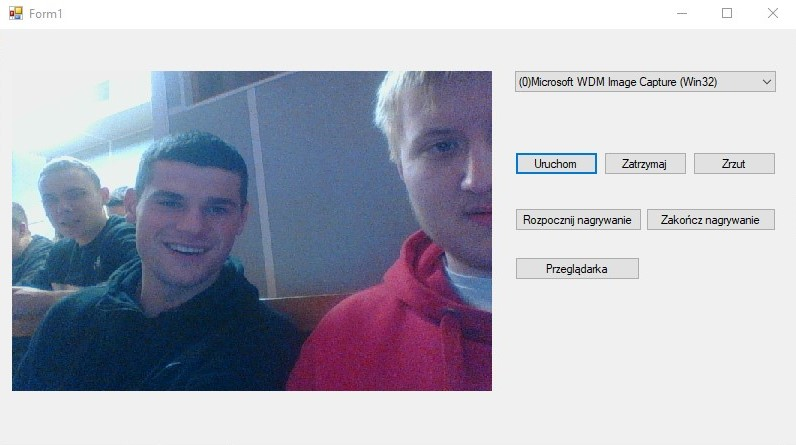
\includegraphics[scale=0.7]{okno}
\begin{center}
\begin{normalsize}
\textit{Rysunek 1. Interfejs aplikacji}
\end{normalsize}
\end{center}
\begin{lstlisting}
using [...]

namespace CameraForms
{
    public partial class Form1 : Form
    {
        WebCam oWebCam;
        public Form1()
        {
                InitializeComponent();
        }

        private void Form1_Load(object sender, EventArgs e)
        {
                oWebCam = new WebCam();
                oWebCam.Container = pictureBox1;
                oWebCam.ComboBox = comboBox1;
                oWebCam.Load();
        }


        //Rozpoczecie polaczenia
        private void button1_Click(object sender, EventArgs e)
        {
            oWebCam.OpenConnection();
        }
        
        
        //Wlaczenie kamerki w przegladarce, krzystajac z pliku HTML
        private void button2_Click(object sender, EventArgs e)
        {
            Process.Start("file:///C:/Users/DELL/Desktop/ Politechnika/obraz.html");
        }
        //
        private void button3_Click(object sender, EventArgs e)
        {
            oWebCam.Dispose();
        }
        //Zrobienie screenshota
        private void button4_Click(object sender, EventArgs e)
        {
            oWebCam.SaveImage();
        }
        //Rozpoczecie nagrywania
        private void button5_Click(object sender, EventArgs e)
        {
            oWebCam.StartRecording();
        }
        //Zakonczenie nagrywania
        private void button6_Click(object sender, EventArgs e)
        {
            oWebCam.StopRecording();
        }
    }
}
\end{lstlisting}
\subsection{Funkcje wykonywalne}
\begin{lstlisting}
using [...]

namespace CameraForms
{
    public class WebCam : IDisposable
    {
        // Stale sluzace przeciazaniu niezarzadzanych kodow
        // Kazda stala reprezentuje stan

        private const short WM_CAP = 0x400;
        private const int WM_CAP_DRIVER_CONNECT = 0x40a;
        private const int WM_CAP_DRIVER_DISCONNECT = 0x40b;
        private const int WM_CAP_EDIT_COPY = 0x41e;
        private const int WM_CAP_SET_PREVIEW = 0x432;
        private const int WM_CAP_SET_OVERLAY = 0x433;
        private const int WM_CAP_SET_PREVIEWRATE = 0x434;
        private const int WM_CAP_SET_SCALE = 0x435;
        private const int WS_CHILD = 0x40000000;
        private const int WS_VISIBLE = 0x10000000;
        const int WM_CAP_DLG_VIDEOFORMAT = WM_CAP + 41;
        const int WM_CAP_DLG_VIDEOSOURCE = WM_CAP + 42;
        private const int WM_CAP_FILE_SET_CAPTURE_FILE = WM_CAP + 20;
        private const int WM_CAP_SEQUENCE = WM_CAP + 62;
        private const int WM_CAP_STOP = WM_CAP + 68;
        private const int WM_CAP_FILE_SAVEAS = WM_CAP + 23;

        //zapis bitmapy
        const int WM_CAP_SAVEDIB = WM_CAP + 25;
        private const short SWP_NOMOVE = 0x2;
        private short SWP_NOZORDER = 0x4;
        private short HWND_BOTTOM = 1;

        private Timer _timer;

        //Ta funkcja umozliwia wylistowanie urzadzen kamery internetowej
        [DllImport("avicap32.dll")]
        protected static extern bool capGetDriverDescriptionA(short wDriverIndex,
            [MarshalAs(UnmanagedType.VBByRefStr)]ref String lpszName,
           int cbName, [MarshalAs(UnmanagedType.VBByRefStr)] ref String lpszVer, int cbVer);

        //Ta funkcja umozliwia utworzenie okna, aby mozna bylo je wyswietlic np w PictureBox
        [DllImport("avicap32.dll")]
        protected static extern IntPtr capCreateCaptureWindowA([MarshalAs(UnmanagedType. VBByRefStr)] ref string
    	lpszWindowName,
            int dwStyle, int x, int y, int nWidth, int nHeight, int hWndParent, int nID);

        //Ta funkcja umozliwia zmiane pozycji okna
        [DllImport("user32")]
        protected static extern int SetWindowPos(IntPtr hwnd, int hWndInsertAfter, int x, int y, int cx, int cy, int wFlags);

        //Ta funkcja umozliwia wyslanie odpowiedniej wiadomosci do okna
        [DllImport("user32", EntryPoint = "SendMessageA")]
        protected static extern int SendMessage(IntPtr hwnd, int wMsg, int wParam, [MarshalAs(UnmanagedType.AsAny)] object
    	lParam);

        [DllImport("user32", EntryPoint = "SendMessageA")]
        protected static extern int SendMessage(IntPtr hwnd, int wMsg, bool wParam, [MarshalAs(UnmanagedType.AsAny)] object
            lParam);

        //Ta funkcja pozwala zniszczyc okno
        [DllImport("user32")]
        protected static extern bool DestroyWindow(IntPtr hwnd);

        // ID urzadzenia
        int DeviceID = 0;
        // Wskaznik uchwytu dla okna podgladu
        private IntPtr hHwnd;
        //Lista urzadzen
        ArrayList ListOfDevices = new ArrayList();

        //Wstawienie obrazka
        public PictureBox Container { get; set; }
        public ComboBox ComboBox { get; set; }

        // Polaczenie z urzadzenem .
        /// Zaladowanie listy urzadzen
        public void Load()
        {
            string Name = String.Empty.PadRight(100);
            string Version = String.Empty.PadRight(100);
            bool EndOfDeviceList = false;
            short index = 0;
            _timer = new Timer { Interval = (200) };
            _timer.Elapsed += new ElapsedEventHandler(TimerTick);
            _timer.Enabled = true;
            _timer.Start();
            // ladowanie wszsytkich dostepnych urzadzen do listy
            do
            {
                // pobranie nazwy i wersji
                EndOfDeviceList = capGetDriverDescriptionA(index, ref Name, 100, ref Version, 100);
                // Jesli jest urzadzenie, to dodanie jego nazwy do listy
                if (EndOfDeviceList) ListOfDevices.Add("(" + index + ")" + Name.Trim());
                index += 1;
            }
            while (!(EndOfDeviceList == false));

            ComboBox.Items.AddRange(ListOfDevices.ToArray());
            ComboBox.SelectedIndex = 0;
        }

        /// Funkcja do wyswietlania danych wejsciowych z urzadzenia przechywtujacego wideo
        /// nalezy utworzyc okno przechwytywania.
        public void OpenConnection()
        {
            string DeviceIndex = Convert.ToString(DeviceID);
            IntPtr oHandle = Container.Handle;

            // Otwarcie podgladu w PictureBox .
            // Tworzenie podrzednego okna, aby mozna bylo je wyswietlic w PictureBox

            hHwnd = capCreateCaptureWindowA(ref DeviceIndex, WS_VISIBLE | WS_CHILD, 0, 0, 1280, 720, oHandle.ToInt32(), 0);

            // Polaczenie z urzadzeniem
            if (SendMessage(hHwnd, WM_CAP_DRIVER_CONNECT, 0, 0) != 0)
            {
                // Ustawienie skali podgladu
                SendMessage(hHwnd, WM_CAP_SET_SCALE, true, 0);
                // Ustawienie czestotliwosci odswiezania podgladu
                SendMessage(hHwnd, WM_CAP_SET_PREVIEWRATE, 66, 0);

                // Rozpoczecie przegladanie obrazu z kamery
                SendMessage(hHwnd, WM_CAP_SET_PREVIEW, true, 0);

                // Dopasowanie okna do ramki graficznej
                SetWindowPos(hHwnd, HWND_BOTTOM, 0, 0, Container.Width, Container.Height, SWP_NOMOVE | SWP_NOZORDER);
            }
            else
            {
                // Blad przy polaczeniu urzadzenia
                DestroyWindow(hHwnd);
            }
        }

        public void Settings()
        {
            SendMessage(hHwnd, WM_CAP_DLG_VIDEOFORMAT, DeviceID, 0);
        }


        public void ImageSettings()
        {
            SendMessage(hHwnd, WM_CAP_DLG_VIDEOSOURCE, DeviceID, 0);
        }

        void CloseConnection()

        {
            SendMessage(hHwnd, WM_CAP_DRIVER_DISCONNECT, DeviceID, 0);
            // zamkniecie okna
            DestroyWindow(hHwnd);
        }

        public void StartRecording()
        {
            SendMessage(hHwnd, WM_CAP_FILE_SET_CAPTURE_FILE, 0, @"C:\Users\DELL\Desktop\Politechnika\Semestr 5\Urzadzenia peryferyjne\LAB\UP_Kamera\nagranie.avi");
            SendMessage(hHwnd, WM_CAP_SEQUENCE, DeviceID, 0);
        }

        public void StopRecording()
        {
            SendMessage(hHwnd, WM_CAP_FILE_SAVEAS, DeviceID, @"C:\Users\DELL\Desktop\Politechnika\Semestr 5\Urzadzenia peryferyjne\LAB\UP_Kamera\nagranie.avi");
            SendMessage(hHwnd, WM_CAP_STOP, DeviceID, @"C:\Users\DELL\Desktop\Politechnika\Semestr 5\Urzadzenia peryferyjne\LAB\UP_Kamera\nagranie.avi");
        }
        public void SaveWebImg()
        {
            SendMessage(hHwnd, WM_CAP_SAVEDIB, DeviceID, @"C:\Users\DELL\Desktop\Politechnika\doWebu.jpg");
        }
        public void SaveImage()
        {
            SendMessage(hHwnd, WM_CAP_SAVEDIB, DeviceID, @"C:\Users\DELL\Desktop\Politechnika\Semestr 5\Urzadzenia peryferyjne\LAB\UP_Kamera\zdjecie.jpg");
        }

        void TimerTick(object sender, ElapsedEventArgs e)
        {
            SaveWebImg();
        }
        // Ta funcja konczy polaczenie z urzadzeniem
        #region IDisposable Members

        public void Dispose()
        {
            CloseConnection();
        }
        #endregion
    }
}



\end{lstlisting}

\subsection{Plik HTML}
\begin{lstlisting}
<html>
	<head>
	</head>
	<body>
		<img src="doWebu.jpg"/>
		<meta http-equiv="refresh" content="0.2">
	</body>
</html>
\end{lstlisting}
\end{adjustwidth}
\section{Wnioski}
Podczas ćwiczenia poznaliśmy podstawową obsługę kamery USB i funkcje takie jak nagrywanie, przechwytywanie obrazu, czy wyświetlanie obrazu na stronie internetowej. AVICAP32.dll mimo, iż jest bardzo starą biblioteką, umożliwił nam sprawne wykonanie wyżej wymienionych zadań.
\section{Bibliografia}
\begin{itemize}
\item Dokumentacja Microsoftu:
\\
$https://docs.microsoft.com/en-us/windows/desktop/api/vfw/$
\end{itemize}
\end{document}